% Options for packages loaded elsewhere
\PassOptionsToPackage{unicode}{hyperref}
\PassOptionsToPackage{hyphens}{url}
%
\documentclass[
]{book}
\usepackage{amsmath,amssymb}
\usepackage{lmodern}
\usepackage{iftex}
\ifPDFTeX
  \usepackage[T1]{fontenc}
  \usepackage[utf8]{inputenc}
  \usepackage{textcomp} % provide euro and other symbols
\else % if luatex or xetex
  \usepackage{unicode-math}
  \defaultfontfeatures{Scale=MatchLowercase}
  \defaultfontfeatures[\rmfamily]{Ligatures=TeX,Scale=1}
\fi
% Use upquote if available, for straight quotes in verbatim environments
\IfFileExists{upquote.sty}{\usepackage{upquote}}{}
\IfFileExists{microtype.sty}{% use microtype if available
  \usepackage[]{microtype}
  \UseMicrotypeSet[protrusion]{basicmath} % disable protrusion for tt fonts
}{}
\makeatletter
\@ifundefined{KOMAClassName}{% if non-KOMA class
  \IfFileExists{parskip.sty}{%
    \usepackage{parskip}
  }{% else
    \setlength{\parindent}{0pt}
    \setlength{\parskip}{6pt plus 2pt minus 1pt}}
}{% if KOMA class
  \KOMAoptions{parskip=half}}
\makeatother
\usepackage{xcolor}
\usepackage{longtable,booktabs,array}
\usepackage{calc} % for calculating minipage widths
% Correct order of tables after \paragraph or \subparagraph
\usepackage{etoolbox}
\makeatletter
\patchcmd\longtable{\par}{\if@noskipsec\mbox{}\fi\par}{}{}
\makeatother
% Allow footnotes in longtable head/foot
\IfFileExists{footnotehyper.sty}{\usepackage{footnotehyper}}{\usepackage{footnote}}
\makesavenoteenv{longtable}
\usepackage{graphicx}
\makeatletter
\def\maxwidth{\ifdim\Gin@nat@width>\linewidth\linewidth\else\Gin@nat@width\fi}
\def\maxheight{\ifdim\Gin@nat@height>\textheight\textheight\else\Gin@nat@height\fi}
\makeatother
% Scale images if necessary, so that they will not overflow the page
% margins by default, and it is still possible to overwrite the defaults
% using explicit options in \includegraphics[width, height, ...]{}
\setkeys{Gin}{width=\maxwidth,height=\maxheight,keepaspectratio}
% Set default figure placement to htbp
\makeatletter
\def\fps@figure{htbp}
\makeatother
\setlength{\emergencystretch}{3em} % prevent overfull lines
\providecommand{\tightlist}{%
  \setlength{\itemsep}{0pt}\setlength{\parskip}{0pt}}
\setcounter{secnumdepth}{5}
\usepackage{booktabs}
\usepackage{amsthm}
\makeatletter
\def\thm@space@setup{%
  \thm@preskip=8pt plus 2pt minus 4pt
  \thm@postskip=\thm@preskip
}
\makeatother
\ifLuaTeX
  \usepackage{selnolig}  % disable illegal ligatures
\fi
\usepackage[]{natbib}
\bibliographystyle{apalike}
\IfFileExists{bookmark.sty}{\usepackage{bookmark}}{\usepackage{hyperref}}
\IfFileExists{xurl.sty}{\usepackage{xurl}}{} % add URL line breaks if available
\urlstyle{same} % disable monospaced font for URLs
\hypersetup{
  pdftitle={The Calvin University Mathematics Department},
  pdfauthor={Michael Stob},
  hidelinks,
  pdfcreator={LaTeX via pandoc}}

\title{The Calvin University Mathematics Department}
\author{Michael Stob}
\date{2023-04-25}

\begin{document}
\maketitle

{
\setcounter{tocdepth}{1}
\tableofcontents
}
\hypertarget{introduction}{%
\chapter{Introduction}\label{introduction}}

Calvin University opened in 1876 as a theological school to train ministers for the Christian Reformed Church. The program included four years of preparatory studies (the literary department) and two years of theological studies. The preparatory studies were essentially equivalent to a high-school education. In 1884, the institution began admitting other students to the literary department, including prospective teachers. Eventually the preparatory program would be offered in four tracks: Seminary Preparatory, Classical, Modern Classical, and Teachers' Preparatory. By 1906, the college offered two years of general work beyond the four-year preparatory program and became known as ``Calvin Junior College.''

The 1920-21 academic year opened with the institution offering a four-year program (beyond the preparatory school) for the first time. Its completion resulted in the A.B. degree. The college opened its doors with William Rinck as its only mathematics professor. Rinck also served as the college's registrar in that first year. Rinck was not new to Calvin having spent the previous 15 years teaching in the preparatory school and the junior college.

In the next several chapters, I tell my version of the story of the first hundred years (1920-2020) of the mathematics department. Of course there are many different ways to tell that story. Certainly a lot depends on the documentation at hand. I am relying principally on two sources. The first is college catalogs. All 100 of the college catalogs are available on-line through Calvin's Office of Student Success. The catalogs are indispensable for documenting the faculty and curriculum. The second source is my own recollection (enhanced by my personal files). I have been associated with the mathematics department for exactly half of those 100 years having arrived as freshman in 1970 to take an Honors Calculus class taught by Larry Nyhoff. Additionally, I was privileged to be a colleague of Carl Sinke and Paul Zwier whose association with the department went back 20 years before mine and who were perfectly capable of regaling us younger faculty with stories of what it was like in the (good?) old days.

I have chosen to divide the 100 years into four eras. These span the periods 1920-1960, 1960-1980, 1980-2000, and 2000-2020. Of course divisions such as these are artificial just as is the sorting of people into generations (Boomers, Gen X, Millenials, etc.). Change in an academic department is not exactly a continuous function. Each academic year serves as a sort of a jump discontinuity with new students, new faculty, and perhaps curricular change. The divisions that I have made correspond to major curricular shifts. Of course change was more gradual than the bright lines that I have drawn suggest. Some might want to change these boundaries or add eras. But it seems to me that looking at the department through the lens of the four themes that I propose adds to understanding beyond what simply a year to year recounting of people and events might do. Anyway, it's my story so I'll tell it my way.

The next four chapters cover the four eras that I have defined above. But,
in thinking about this broad history of the department, I identified several issues and themes that deserved separate treatment. These are covered in later chapters.

I have used the catalog as my ``source of truth'' concerning faculty and curriculum. There are a couple of causes of systematic errors in relying on the catalog for faculty information. First, the catalog for an academic year was necessarily published before the school year began. Before 1950, the catalog was published in the spring of the preceding academic year. It was called the Yearbook and contained information on the current academic year as well as the calendar and courses for the upcoming year. In later years, the catalog was published sometime in the summer. In either case, the listing of faculty did not necessarily reflect final hiring decisions made in the spring. Second, the definition of membership on the faculty changed over time. In later years, particularly after 1970, the college used many faculty members in one- or two-year term positions. These faculty members had official faculty appointments and were listed, whenever possible, as members of the faculty in the catalog. In earlier years, faculty membership was held somewhat more tightly so that persons teaching in a department might not be listed as members of the faculty. For example, the 1955 catalog list two persons as teaching in mathematics who are not listed in the official list of faculty members in the catalog. Part-time instructors were usually not mentioned in the catalog at all. The catalog is, of couse, more dependable as regards curricular change since the main purpose of a college catalog is to give the ``official'' descriptions of courses and programs. Even so, the catalog is a better indicator of when courses were introduced than when they were last offered. Courses sometimes stayed on the books long after their last offering.

\hypertarget{the-service-department}{%
\chapter{1920-1960: The Service Department}\label{the-service-department}}

\hypertarget{the-college-in-1920}{%
\section{The College in 1920}\label{the-college-in-1920}}

The college opened in 1920 with 122 students, 14 of them female. The catalog actually lists the names, local addresses, and hometowns of all of these students. Forty-four of these students came from out of state, including from states as far as Washington, Montana, and South Dakota. Students paid tuition which depended on their home state. Tuition was \$15 a semester for those students from the midwest and half that for students from west of the Missippi or east of Ohio. Students from Montana, Colorado, New Mexico, or further west paid no tuition. There was a dormitory but most students lived with a host family for around \$7 a week.

There were 20 faculty members on the faculty roster listed in the catalog (including President John Hiemenga). One faculty member had a Ph.D.~(Peter Hoekstra in History). There was also one female faculty member, Nelly Bosma, who was an Instructor in Biology. William Rinck was the sole faculty member in mathematics. Tragically, in his very first semester of the new four-year college, Professor Rinck died in an auto accident along with his young son. He was replaced by James ``Sleepy'' Nieuwdorp who had started the year as an instructor in chemistry. Nieuwdorp was to remain in the mathematics department until 1944. For most of those years he was the only mathematics instructor.

The college offered an A.B. degree with a curriculum loosely patterned on that of the Free University of Amsterdam. To receive this degree, students completed 120 hours including 54 hours of what we now call general education and 66 hours of courses chosen from three different groups. (The groups were, roughly, Languages and Literature, Science and Mathematics, and Social Sciences and Philosophy.) Incredibly, 36 of the 87 courses in the 1920 catalog were foreign language courses (Greek, Latin, Dutch, Hebrew, German, and French).
There were prescribed programs for pre-seminary, pre-medicine (three years), pre-engineering (two years), and pre-law (three years). It was still the case that teachers generally stopped after the preparatory school (high school). The college would introduce a two-year ``normal'' course the next year. There was one pedagogical methods course taught in the preparatory school. Students other than pre-seminary students wanting a four year degree were required to choose a major group and a minor group and complete at least 24 hours in the major group and 20 in the minor group. This basic structure of the major and minor requirements continued until the 1967-68 year when the college introduced the 4-1-4 calendar and radically redesigned the curriculum. The required number of hours in the major and minor gradually increased over these four decades so that by 1960, students were required to choose a 24 hour major in one department, a 12-hour minor in the same group, and 18 hours in a second group.

\hypertarget{mathematics-in-1920}{%
\section{Mathematics in 1920}\label{mathematics-in-1920}}

The mathematics department offered eight different courses.

\begin{figure}

{\centering 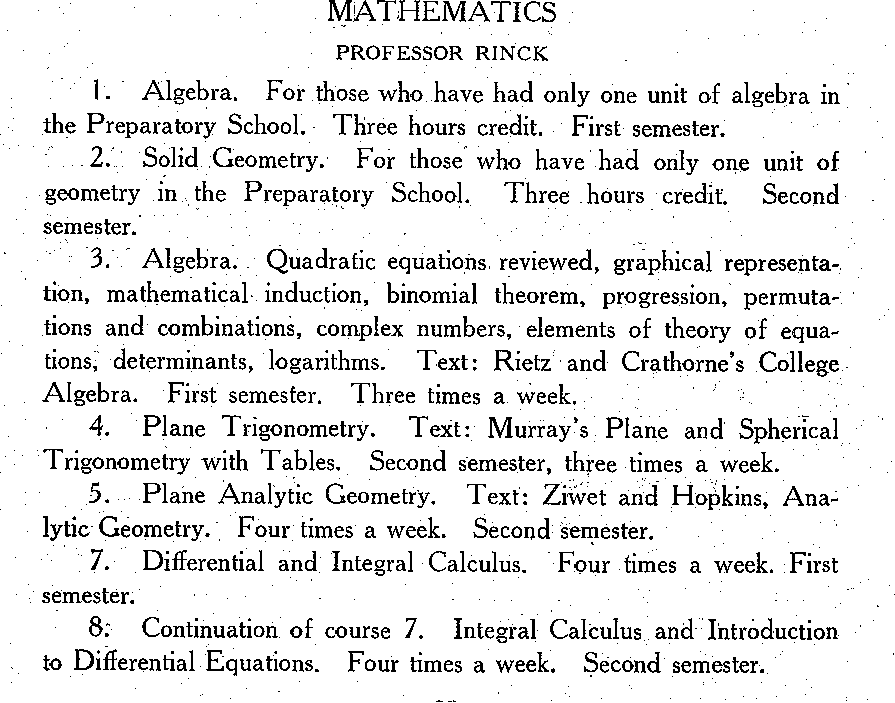
\includegraphics[width=12.43in]{images/1920Program} 

}

\caption{1920 mathematics offerings from the catalog}\label{fig:1920curr}
\end{figure}

Not listed here (in error) is course 6, a continuation of course 5, which appears in the 1921 catalog. Courses 7 and 8 were new to the college, but course 1 and course 2 were preparatory school courses and courses 3-6 were taught previously in the junior college.
All these courses would continue to be offered until the late 1950s (with different numbering schemes).
The pre-engineering students were expected to take courses 5, 6, 7, and 8 in their two years and this prepared them to transfer to the University of Michigan. Until the college introduced a four-year engineering program in 1985, this path of two (later, three) years at Calvin followed by two at Michigan would remain a popular path for Calvin students wanting to be engineers.

The two-course sequence in analytic geometry was substantial (some might say tedious). In the 1970s, Carl Sinke would lament the lack of analytic geometry knowledge of his calculus students. He would have taken course 5 and 6 in the late 1940s.
A typical set of problems from the text on analytic geometry indicates the flavor of the work in courses 5 and 6.

\begin{figure}

{\centering 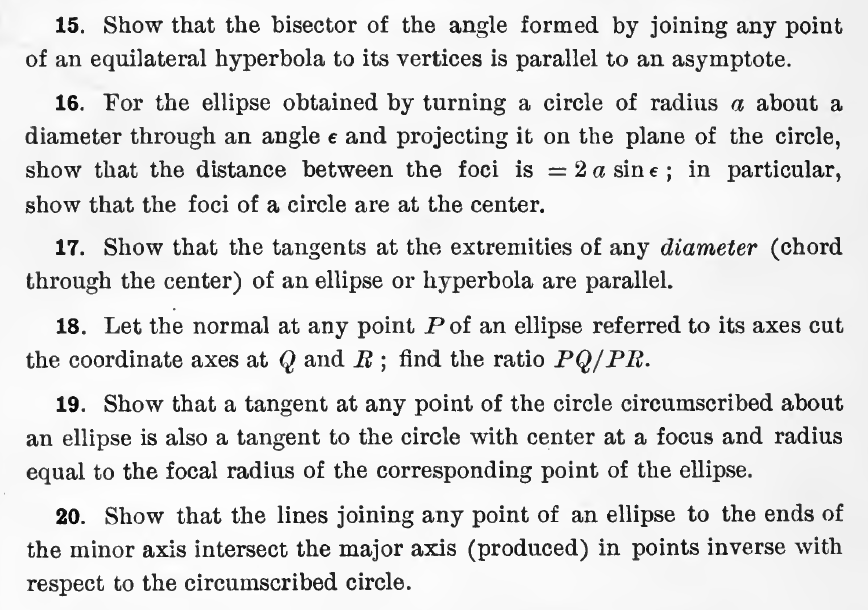
\includegraphics[width=12.06in]{images/ellipseandhyperbola} 

}

\caption{Problems from Ziwet and Hopkins, ellipses and hyperbolas }\label{fig:analytgeom}
\end{figure}

\hypertarget{the-nieuwdorp-years}{%
\section{The Nieuwdorp Years}\label{the-nieuwdorp-years}}

Sleepy Nieuwdorp (as he was called by former students and colleagues) took over from Rinck in the fall of 1920 and he was to serve as the only faculty member for the next twenty years until Muyskens joined him in 1940. In the first few years that he was with the department, Nieuwdorp introduced several new courses. In 1923 the college added courses in Differential Equations and the Theory of Equations. In 1923, the college also introduced a two-year teacher preparation sequence and so the department added the Teacher's Course, a course in mathematics for prospective secondary teachers. In 1926, the department added courses in Solid Analytic Geometry and Projective Geometry. The curriculum would not change again until 1936 when the first statistics course was offered.

Students ``majored'' in mathematics from the very beginning of the college. The 1940 catalog definition of major indicates that a major consists of at least 21 hours. No particular courses are required or specified. The 1940 list of courses shows the orignal eight courses (renumbered) and the five additional courses added over the first two decades.

\begin{figure}

{\centering 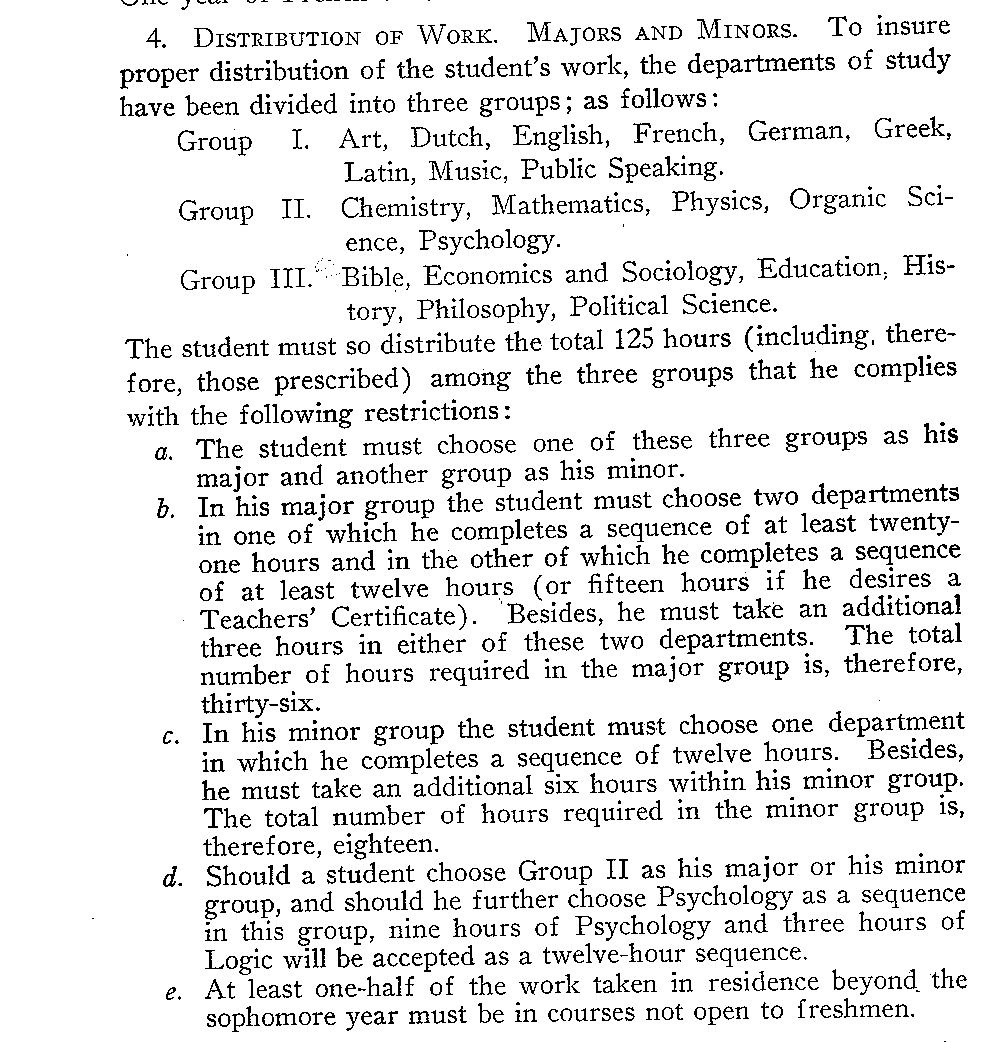
\includegraphics[width=13.68in]{images/1940MajorDef} 

}

\caption{1940 Graduation Requirements}\label{fig:1940cat}
\end{figure}

\begin{figure}

{\centering 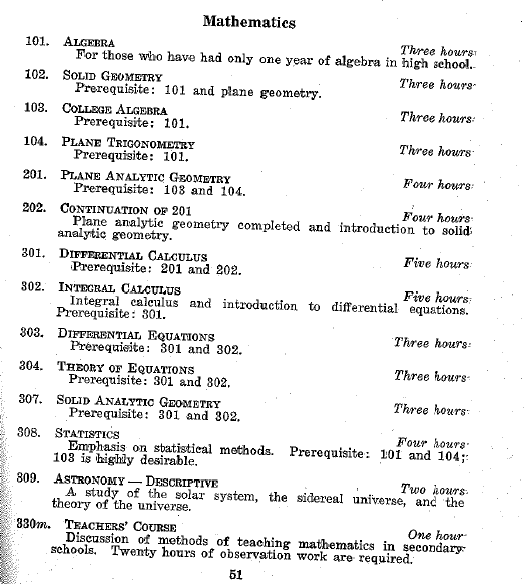
\includegraphics[width=0.6\linewidth]{images/1940Math} 

}

\caption{1940 mathematics offerings from the catalog}\label{fig:1940math}
\end{figure}

\hypertarget{the-muyskens-and-tuls-department}{%
\section{The Muyskens and Tuls Department}\label{the-muyskens-and-tuls-department}}

Albert Muyskens joined Nieuwdorp in the fall of 1940. Muyskens was an alum of the junior college, graduating in 1917. He had been on the faculty as an instructor in Physical Education since 1936. He would coach the varsity basketball team from 1936-1945, attaining a 71\% winning percentage. Nieuwdorp retired in 1944 and John Tuls would join Muyskens in 1946. Tuls was the first graduate of the college to teach in the department, having graduated in 1928.\\
These two would serve as the mathematics department for the rest of this ``era.''
While enrollment was increasing at a rapid rate after the war (the college enrollment was 690 in the fall of 1945 and 2,016 in 1960) and more students were majoring in mathematics (there were more than 20 majors a year graduating each year in the 1950s), the departments curriculum would remain almost unchanged. The only courses added in the 1940s were a spherical trigonometry course that was offered sporadically from 1945 through 1958 and a Business Mathematics course that was added in 1948. An Advanced Calculus course was added in 1958 but it was only taught twice.

\hypertarget{the-golden-years}{%
\chapter{1960 -1980 The Golden Years}\label{the-golden-years}}

There are several reasons why 1960 (or thereabout) represents a natural division in the evolution of the department. First, rapid enrollment increases meant that there were more students to take mathematics and therefore more faculty positions available. College enrollment was only 690 in 1945-46 but grew steadily after the war so that in 1960 enrollment topped 2,000 for the first time. In just five more years, enrollment was to be almost 3,000. Second, to fill the positions open due to increased enrollment, the college was regularly hiring new faculty and, contrary to previous custom, many of these had Ph.D.~degrees. Carl Sinke in 1957 and Paul Zwier in 1960 joined Muyskens and Tuls, doubling the size of the department. Sinke and Zwier were the first mathematics faculty members with doctoral degrees having both earned Ph.Ds. from Purdue and they came with fresh ideas concerning curriculum and pedagogy.

The third reason for identifying 1960 as a watershed year is an external force -- Sputnik. In 1957, the Soviet Union successfully launched a satellite that orbited the earth. This event shocked the nation's scientific establishment as it realized that the U.S. was not necessarily preeminent in science and mathematics. The nation immediately invested in improving science and mathematics education. The National Defense Education Act of 1958 established many programs designed for the ``expansion and improvement of educational programs to meet critical national needs'' and was focused on science, mathematics, and foreign language instruction. The Act set up a federal student loan program for higher education and also provided grants to states for developing programs to strengthen mathematics, science, and foreign language instruction. High quality and modern science texts were created for high school students in the 1960s. The ``new mathematics'\,' reforms were introduced at all levels. In fact, in the early 1960s Sinke and Zwier ran several NSF-funded summer workshops for teachers at Calvin. And many high school and elementary school teachers participated in NSF-sponsored summer workshops in science and mathematics. By the late 1960s, the physics and mathematics majors at Calvin had become enormously popular.

\begin{figure}

{\centering 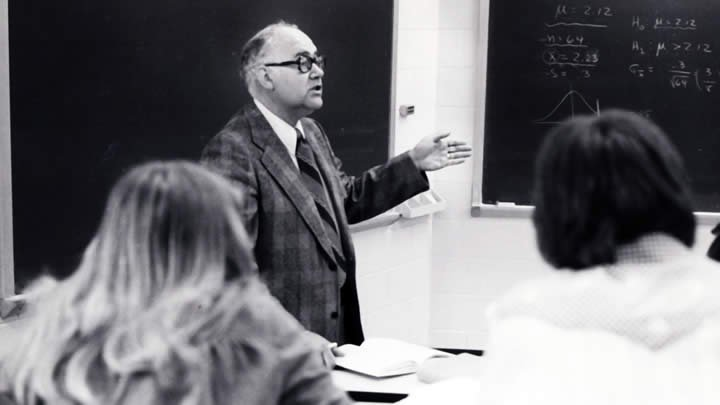
\includegraphics[width=0.5\linewidth]{images/sinke1} 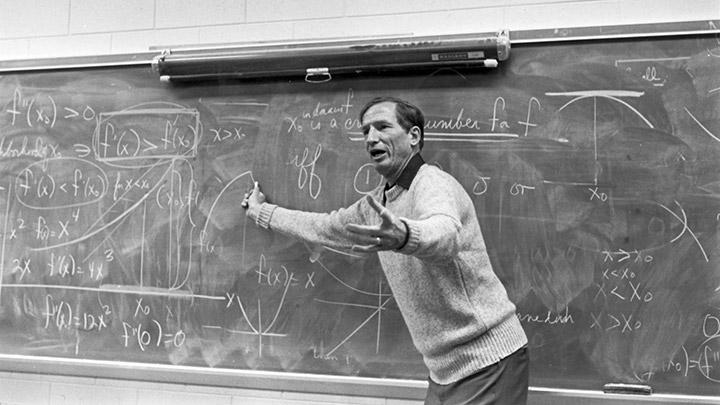
\includegraphics[width=0.5\linewidth]{images/zwier} 

}

\caption{Carl Sinke and Paul Zwier in action}\label{fig:sinkzwier}
\end{figure}

\hypertarget{faculty-growth}{%
\section{Faculty Growth}\label{faculty-growth}}

The 1960 school year started with Muyskens, Tuls, Zwier and Sinke on the faculty. Muyskens would retire in 1962.
Over the course of the next decade, the department would add George Van Zwalenberg (PhD, Berkeley, 1968), Paul Boostra (Ph D, Michigan State,1970), Jack Kuipers (MSE, Michigan, 1966) , Larry Nyhoff (Ph D, Michigan State, 1969) , and Sandford Leestma (PhD, New Mexico State, 1969). All of these were Calvin graduates of the early 1960s. Boonstra was the first hire in the area of mathematics education and would go on to supervise hundreds of prospective secondary school mathematics teachers in his 20-year tenure in the department. Nyhoff and Leestma were trained in mathematics but would play an instrumental role later in establishing the computer science program at Calvin (a story told in the next chapter). Jack Kuipers, the only non PhD in the group, had a masters degree in electrical engineering and taught applied mathematics, often to prospective engineers. Tuls retired in 1973, but all these other faculty members were still around in 1980.

Late in the 1970s, Jom Jager (Ph D, Chicago, 1971), Daryl Brink (Ph D, Michigan State, 1973), and Gerard Venema (Ph D, Utah, 1975) joined the department. Also through the late 1970s, the department began to rely on term (non-tenure-track) appointments to expand the faculty without making long-term commitments. Thus, during the 1979-80 academic year, there were 9 faculty on tenure-track appointments and 4 on term appointments. (Brink was on a term appointment that would later be converted to tenure-track.)

\hypertarget{towards-a-more-modern-curriculum}{%
\section{Towards a More Modern Curriculum}\label{towards-a-more-modern-curriculum}}

Of the courses being taught in 1959, all but three of them had been introduced in the 1920s. These three were the statistics course introduced in 1936, the business mathematics course introduced in 1948, and an advanced calculus course introduced in 1957. Of the eight original courses, seven were still being offered. The department (probably primarily Sinke and Zwier) realized a major overhaul was in order. In 1960, the department introduced a Mathematical Statistics course (taught primarily by Sinke over the next couple of decades) and a Modern Algebra course (taught primarily by Zwier).

In 1961, the department effected a major curriculum revision. The most important change was the elimination of the two course analytic geometry sequence (courses 5 and 6 of 1920). In its place, the calculus sequence was expanded to three courses and analytic geometry was incorporated in all three courses (and the titles of the courses). This effectively made calculus the beginning of the major sequence although a course in college algebra was introduced for those students not prepared for the calculus sequence. (College algebra had been the original course 3 but hadn't been offered since 1952.) The department changed not only the introductory sequence but also added a significant number of offerings at the upper-level for majors including courses in Linear Algebra and Modern Geometry as well as a two course sequence called Advanced Analysis. This two-course sequence initially contained such topics as vector analysis, Stoke's Theorem, series, and complex analysis. The two-course sequence was designed to appeal to engineers and scientists as well as mathematics students and its content evolved over time as the needs of students and the syllabus of the third semester of calculus changed. The current successors of this two-course sequence are the courses in partial differential equations and in complex analysis. The mathematics major in 1961 was defined as the ``new freshman-sophomore sequence'' (three semesters of calculus and one of differential equations) and two additional courses chosen from those numbered 300 or above. This constituted a 24 hour major. Currently, a 24 hour program does not seem like a major but such programs were typical in 1960.

By the end of the 1960s, the college had added five more courses at the 300-level: Topology, Real Analysis, History of Mathematics, Numerical Mathematics, and a second semester of Modern Algebra. In 1963, the college also introduced a course in mathematics for the liberal arts student called ``Elements of Modern Mathematics'' and Sinke and Zwier would write a text for the course.

\begin{figure}

{\centering 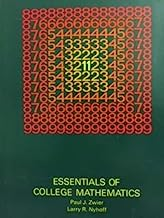
\includegraphics[width=0.5\linewidth]{images/ZwierSinke109} 

}

\caption{Sinke and Zwier text for Mathematics 109}\label{fig:zwiersink}
\end{figure}

\hypertarget{the-4-1-4-plan}{%
\section{The 4-1-4 Plan}\label{the-4-1-4-plan}}

Just as in the Mathematics Department, other departments across campus were hiring young PhDs who were anxious to modernize the curriculum. In 1965, a committee of the faculty chaired by the Nick Wolterstorff who had joined the faculty in 1959 prepared a report called ``Christian Liberal Arts Education.'' This report gave a philosophical argument for a complete overhaul of the college curriculum, academic calendar, and even credit assignment practices. The new calendar had two somewhat shortened semesters and a one-month January term sandwiched in between. Essentially all courses were to carry the same credit (one ``unit'') and students would typically take 4 courses each semester and one intensive course each January. The new curriculum also included a 17-course set of core curriculum requirements. The proposal also formalized the notion of concentration. Students would henceforth be required to complete a concentration (major) of the department's specification. (Previously, students needed only complete 24 hours in a department.) Minors were eliminated although group majors were possible for students desiring breadth.

The 4-1-4 plan went online in 1967. The department defined a major to be nine courses: the three calculus courses, differential equations, abstract algebra, three additional 300-level courses. In 1968, the department added the completion of a junior-senior level interim to the major requirements. Faculty members offered a wide range of interim courses those first few years including such courses as graph theory, number theory, celestial mechanics, differential geometry, philosophy of mathematics, and elementary computer programming.

\hypertarget{new-digs}{%
\section{New Digs}\label{new-digs}}

From 1920 to 1967, the mathematics department was housed in the science building on the Franklin Campus. Beginning in 1962 however, the college gradually relocated to the (current) Knollcrest campus and in 1968 the new science building was opened. (The science building has been added to twice since -- with North Hall and DeVries Hall). The mathematics department had a suite of offices on the first floor. This was the first time faculty members had private offices. There were six offices in the suite and other mathematics faculty members were dispersed throughout the rest of the building. The facilities were important for fostering greater student-faculty interaction. With private offices just around the corner from classrooms, faculty could easily hold office hours and it was not uncommon to see lines in front of the various calculus instructors offices. The mathematics department was to remain in the science building until it outgrew the space available in the early 1980s.

\hypertarget{departmental-traditions}{%
\section{Departmental Traditions}\label{departmental-traditions}}

The 1960s were a time when important departmental traditions and ways of working were solidified. Given the number of mathematics majors, there were enough activity to form a vibrant community and the department worked very intentionally at this. One extraordinarily important tradition is the mathematics department colloquium. Established at least as early as 1967 and always held on Thursday afternoon at 3:30, the colloquium featured a talk often by a visitor from outside Calvin. Refreshments precede the talk. While attendance was not mandatory until the 1980s, many upper-level majors routinely attended and, since there were a lot of majors, SB 101 was often close to full. Several visitors each year came as sort of recruiters for graduate school. This was invaluable for students considering graduate school as it was difficult to get current, dependable information of graduate programs.

Another important tradition is the department picnic. Each fall, the department hosts current mathematics students for a picnic after classes (on a Thursday currently although Friday originally). The tradition is that faculty members supply desserts and side dishes and grill meat. Until cost became prohibitive, the meat was steak (now it's burger and hot dogs).
The picnic was held at the Christian Reformed Recreation Center before it folded which allowed for a faculty-student softball game and touch football. The picnic eventually moved on-campus which helped to improve attendance as finding transportation was not necessary.

Another tradition is the participation of students in mathematical problem-solving competitions. Calvin has had students participating in the Putnam Competition each year since the early 1960s. While participation has decreased over time, in some years Calvin had more than 30 participants in this competition. A highlight was the 1973 team of Steve Haan, David VanBaak, and David Cok (all physics majors) which finished twentieth. Other competitions have been added over the years including the Lower Michigan Mathematics Competition (started by Kalamazoo College), the Fall Take-Home Challenge (started by Alma College), and the International Competition in Modeling. A Calvin team of David Cole, Loren Haarsma, and Jack Snoeyink received the highest award in the first edition of the International Competition in Modelling in 1985.

\hypertarget{computer-science-and-professional-programs}{%
\chapter{1980-2000 Computer Science and Professional Programs}\label{computer-science-and-professional-programs}}

There is no question that 1980 is a logical marker for a turn in direction of the department towards computer science. Larry Nyhoff and Sandy Leestma had been teaching computer programming courses for a decade. Three (half-)courses -- Computer Programming for Business, for Social Sciences, and for Sciences -- were popular enough that people outside the department had to be dragooned into teaching a section or so. Mike Stob taught a section as a senior undergraduate. Then, in 1980, the department launched a computer scene major. The major was heavily mathematics-based. The five required courses included three semesters of calculus, a half credit course in Fortran programming, and a computer science course in Discrete Mathematical Structures. Six elective courses were required but there were only three computer science courses available for those electives -- Computer Organization, Data Structures, and Compiler Design. There were enough mathematics and physics electives included so that a student could in principle receive a computer science degree with just 1.5 computer science courses, one of which (discrete math) was really just another mathematics course! As there was so much mathematics required in the computer science major, most computer science majors were double majors.

Just as new faculty and a major curricular revision propelled the mathematics department into a new era in 1961, new hires and a major curricular revision in 1982 launched the computer science program.

\hypertarget{the-1982-computer-science-revision}{%
\section{The 1982 Computer Science Revision}\label{the-1982-computer-science-revision}}

In 1982-83, enough computer science courses were introduced so that a full major in computer science could be offered without the need to count several mathematics courses in the major. Importantly, a two-course sequence in programming was introduced so that the major finally had a robust starting sequence. Initially, the computer language used was Pascal but this would change over the years to Modula 2, C++, and Java. Also, a unique course (at the time) called Perspectives in Computing, was introduced. This senior-level, seminar course placed special emphasis on social implications and ethical and legal issues in computing. While ``capstone'' courses such as this one are common now due to changing core requirements, they were still somewhat of a novelty when this one was introduced. By 1987--88 there were enough computer science courses so that students had significant choices among electives and could choose one of four emphases in their program. Several courses were of a more applied nature.

In 1995, the department thoroughly revised the major. New courses were introduced and some deleted. The areas of emphases were reduced from five to two (computing and software engineering). A ``practical experience'' requirement was introduced. The general result of these changes was to make a somewhat more ``applied'\,' major while still emphasizing general principles rather than specific technical skills and still being appropriate for graduate-school bound students as well as students immediately entering the
workplace.

In 1996, the department's proposal to split into two departments summarized the previous fifteen years of curricular development this way:

\begin{quote}
In summary, the computer science major of fifteen years ago was very theoretical in nature, relied heavily on mathematics, prepared students appropriately for graduate school, and was taught by mathematicians. It has evolved into a major that has a wide array of options including both theoretical and applied courses, is not necessarily dependent on mathematics, prepares students for a variety of careers as well as graduate school, and is most appropriately taught by faculty with specific, recent training and/or experience in computer science.
\end{quote}

\hypertarget{faculty-hiring-in-the-1980s-and-1990s}{%
\section{Faculty Hiring in the 1980s and 1990s}\label{faculty-hiring-in-the-1980s-and-1990s}}

At the start of the 1980-81 academic year, there were 9 tenure-track faculty members and four faculty members who were on one- or two-year term appointments. Just three of those were prepared to teach computer science. Larry Nyhoff and Sandy Leestma, though mathematicians by training, had spent the decade of the 1970s teaching programming and the college was also paying for them to pursue masters degrees in computer science. Dawn Wolthuis had a masters in computer science and was hired on a two-year term position. Dawn would later go on to direct the computer center (as Calvin Information Technology was then called).

As the computer science offerings grew, it was imperative to find computer scientists to teach them. This proved to be extraordinarily difficult for several reasons. First, computer science PnDs were scarce. Most computer science doctoral programs were relatively new and many graduate institutions didn't have one. Furthermore, PhDs had a lot of opportunities outside of teaching and usually these were considerably more lucrative. Second, Calvin's religious screen was very fine and so the college tended to mostly hire its own graduates. But there were very few alums at that time who had computer science PhD. Third, faculty salaries were entirely based on degree and years of experience. It was difficult to compete with institutions that had negotiating room. A few candidates were lost to other institutions because of salary alone. Fourth, Calvin expected a PhD for tenure-track positions so strong candidates with only Masters degrees could only be offered term positions. Fifth, Calvin's hiring process was Byzantine. A candidate needed to come to campus three times before receiving an offer -- for a departmental interview, for an interview with the Professional Status Committee, and for an interview with the Board of Trustees. This final interview was in May but potential candidates often had firm offers from other institutions in January.

A final factor complicating the search for computer scientists and for department faculty generally was that the college was being very conservative in creating tenure-track positions. Though the department had teaching capacity for 14 full-time faculty members in 1980, it had just 10 tenure-track positions (one filled by Stob who wouldn't arrive until 1981). This conservatism was caused by the serious fluctuations in enrollment during the 1980s and 1990s. The following graph shows the number of FTIACs (first-time in any college students) over the twenty year period. Each year during this time the college budgeted conservatively, never planning on more that 900 or so FTIACs and this meant that new positions were often at most term positions.

\begin{figure}

{\centering 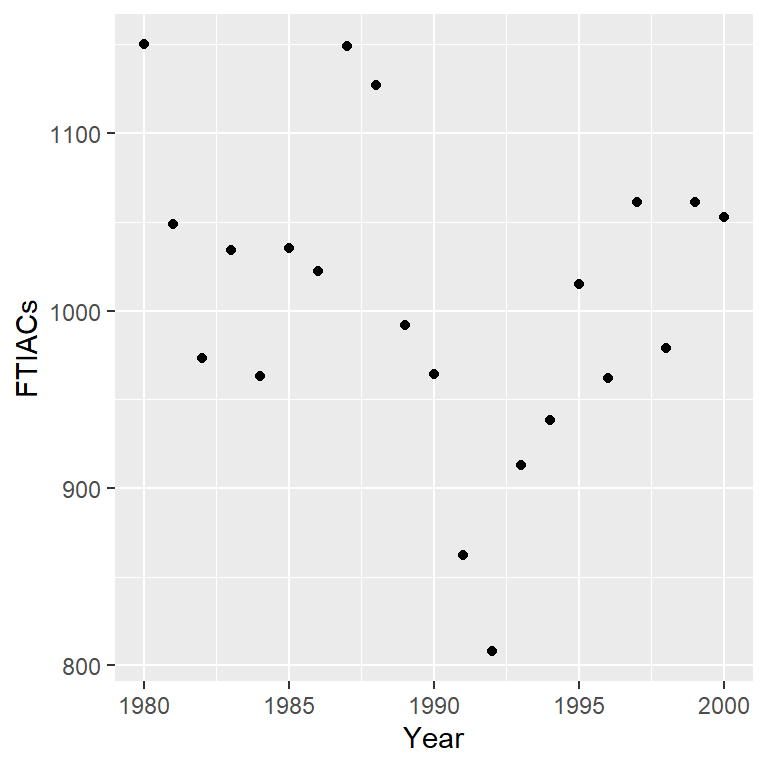
\includegraphics{Calvin-Mathematics_files/figure-latex/FTIACS80s-1} 

}

\caption{Entering First-Year Students (FTIACs)}\label{fig:FTIACS80s}
\end{figure}

All these factors conspired to make it quite difficult to hire computer scientists. But one strategy that turned out to be successful was to hire mathematics PhDs who had retrained as computer scientists. David Laverell actually spent a few years in industry and started in 1984. Jim Bradley came in 1986 and Earl Fife in 1988. In each case, the PhD, even though it was not in computer science, qualified them for tenure-track appointments and their prior experience was honored in determining their starting salary. All three of these faculty members would stay at Calvin for the rest of their career, eventually with joint appointments in mathematics and the eventual computer science department.
Calvin finally hired a PhD computer scientist, Joel Adams, in 1989. The second, Keith Vader Linden, would come in 1996.

While the college enrollment fluctuated, enrollment in the department increased over the two decades. This was due in large part to the increase in mathematics course-taking by students in other departments. The introduction of professional programs with significant mathematics requirements and the addition of mathematics requirements in other programs provided a steady stream of students for the department. (We describe these trends below.) This meant that the department was able to hire. Whereas there were 13 faculty positions in 1980, there were 16 in 1999 (of which four were joint with Computer Science and two were term). Since there were additionally three faculty members in the computer science department, this was really a growth of six positions in total. In fact, the department hired 45 faculty members to either term or tenure-track positions from 1980-1999. (This constant hiring placed considerable burden on the department including the department chair and, inevitably, led to some hires to term positions that weren't especially successful). Retirements in this period included Kuipers (1986), Sinke (1991), Zwier (1996), and Van Zwalenberg (1999). Tragically, Paul Boonstra passed away in 1987 due to leukemia. Fortunately, the department had just hired Gary Talsma to be a second chair in the area of mathematics education so he stepped into the leadership postion immediately.

Tenure-track hires in these two decades included Wayne Dyksen, Jim Bradley, Gene Klassen, David Laverell, Gary Talsma, Jan Koop, Earl Fife, Xiang Dong Ye, John Ferdinands, Yousceek Jeong, Randy Pruim, Rikki Wagstrom, Jim Turner, and Mark Hanisch. While all previous tenure-track hires had been Calvin graduates, only four of these were. All were PhDs and five of these had considerable college teaching experience elsewhere. Koop and Wagstrom were the first two female tenure-track hires. Talsma and Koop were hired to serve the needs of mathematics education. Jeong was a statistician. Fife, Bradley and Laverell were hired primarily to support computer science. Together, these 13 brought considerable diversity, complementary specialty strengths, and some greatly needed consistency among the many term appointees that came and went.
Eight of these 13 would either retire from Calvin or are still teaching in the department.

\hypertarget{moving-again-twice}{%
\section{Moving Again, Twice}\label{moving-again-twice}}

The department had outgrown its original allotment of six offices immediately and by 1980 there was really no place to put new faculty. In 1981, for example, new faculty occupied the offices of faculty on sabbatical that year. There were not enough classrooms in the science building for all the departments teaching there and there were no classrooms particularly appropriate for teaching computer science. Thus in Fall 1982 the department moved to a dormitory, Timmer Hall, a newly constructed addition to Heyns Hall. Timmer was constructed based on anticipated enrollment growth. When that didn't immediately materialize, there was space available. The department was moved to one wing (the Hall was V-shaped with two wings) and occupied the basement and first floor. Female students occupied the second floor above the department and the entire other wing. Having offices in a girls dorm did present a few logistical issues (and one or two awkward moments). The Dean of Women thought it inappropriate for faculty to be in their offices in the evening and some negotiation was necessary. The actual facilities turned out to meet the needs of the department well. Each faculty member had a dorm room (and shared a bathroom with one other faculty member), Two rooms in the basement were repurposed to a small classroom and the mathematics library (which housed current periodicals and back issues). One ``coffee kitchen'' was converted to a department office and the other was retained as a place for faculty to have coffee or lunch. The move to Timmer Hall separated the department from the Science Building so made it more difficult to rely on the division's secretary. Thus, the department hired its first secretary, Bess Exoo. Separated from the Science Building, the department had difficulty finding classrooms to teach its courses. The classroom in the basement of Timmer Hall was appropriate for small classes like Topology and Logic but mathematics classes were offered in every academic building on campus during the Timmer Hall years.

Timmer Hall was temporary. In 1985, the college opened North Hall, an addition to the Science Building. The department moved into the office space on the second floor that it still occupies today. Five new classrooms in North Hall were designed to fit the needs of mathematics teaching. A room was set aside as the ``Faculty Computer Room'' not anticipating that by the time that faculty occupied North Hall, faculty would generally have computers in their offices. A computer classroom was constructed in the basement.

\hypertarget{a-new-department}{%
\section{A New Department}\label{a-new-department}}

In 1996, the Department of Mathematics proposed that it split into two separate departments: the Department of Computer Science and the Department of Mathematics and Statistics. The proposal to the administration put the situation this way:

\begin{quote}
The computer science program has been well-served by being part of the larger Department of Mathematics and Computer Science. The larger size of the Department enabled more people to be involved in program development, faculty development, and student advising. It allowed the department to continue to offer small classesin computer science because of the larger classes in mathematics. (For many years, the student-faculty ratio in the computer science portion of the department offerings was much lower than that of mathematics.) It allowed committee work and administrative responsibilities to be handled by others while the computer science faculty attended to curriculum development. Mathematicians even participated in writing a grant proposal for laboratory facilities for computer science.
\end{quote}

\begin{quote}
However it is also true that the program can now be considered to be a mature one and potentially self-supporting and independent. Student-faculty ratios in the two subdepartments have been nearly equal for the past four years. The current interest in computer science seems more stable than the rather volatile nature
of the interest of the early eighties. Curriculum and advising issues are almost completely independent of those in the mathematics department. Two Ph.D.~computer scientists are now on staff. Except for a need for joint appointments that will exist until the current faculty members that teach in both areas retire and except for some shared resources the
programs can function independently.
\end{quote}

Adams, Vander Linden, and Nyhoff moved to the new department while Bradley, Fife, Laverell, and Leestma received joint appointments to the two departments. With Fife's retirement in 2013, the two departments finally became completely separate.

\hypertarget{the-growth-of-professional-programs}{%
\section{The Growth of Professional Programs}\label{the-growth-of-professional-programs}}

The mathematics department had always been a ``service'' department, serving the needs of other departments and the general education program. But the 1980s saw new professional programs being introduced and ongoing programs reexamining and increasing their mathematics cognate requirements.

The biggest change of this nature was the introduction in 1984 of a four-year engineering degree, a BSE. Calvin had always had pre-engineering students and in 1980 students could find a three-year plan of courses that would prepare them for completing an engineering degree at another institution (often Michigan) in three or four semesters. Upon completing such a program at another school, Calvin awarded such students a Bachelors Degree in Engineering and Letters. This three-year plan included the two-year mathematics sequence (three semesters of calculus and one of differential equations) and a third-year technical elective which could be taken in mathematics. These four or five courses from each engineering student were an important component of the department's overall enrollment. Approximately 30 students a year were completing the three-year program in the early 1980s. By 1984, it became apparent that entry into other schools by transfer was becoming more competitive or, at least, not routine and the Calvin Engineering Department introduced a four-year degree program as an alternative. While the original proposal anticipated that many students would still opt to complete their program at other institutions, immediately essentially all engineering students stayed at Calvin to complete their degree. Calvin graduated its first engineers in the new program in 1985. The four-year program included an advanced mathematics elective so all these students took five mathematics courses. Additionally, since a minor in mathematics could be had with six courses, many engineering students added a sixth mathematics course. Not only were students taking more mathematics but also the program became quite an effective recruiting tool and enrollment increased so that by 1999 there were 115 entering freshmen starting the engineering programming and 302 students overall in the programs.

Increasing enrollment in the engineering department was, of course, a blessing for the department in that it ensured increasing enrollment in mathematics courses though college enrollment and the number of mathematics majors fluctuated. On the other hand, this caused increasing challenges for the department in that the enrollment in several courses became dominated by engineering students and their needs were not always congruent with those of majors in mathematics and the other sciences.

Another professional program that required additional departmental resources was the education program. For many years, the department taught prospective high school mathematics teachers. Paul Boonstra and Gary Talsma were responsible for the supervision of these students in the directed teaching semester and there were as many as a dozen teachers in a given year. But the 1980s saw considerable attention being given to the mathematics preparation of elementary school teachers. Throughout the 1970s and early 1980s, the department was teaching a course intended for elementary teachers. While the course received core credit, it was optional in the program. In 1986, the department introduced a two course sequence, Mathematics 221 and 222 (222 was a half-course) designed to be integrated contents-methods courses for elementary education. Mathematics 221 was roughly arithmetic and 222 was geometry and a little statistics. In 1990, 222 became a full course and from then on all elementary education students took both 221 and 222. By the mid 1990s, the department was offering 6 sections of Mathematics 221 and 5 of Mathematics 222 each year which was just about two FTE of faculty worth of teaching. Jan Koop, a mathematics education specialist, joined the department in 1989 and Talsma and Koop would be the mathematics education team for many years. Others in the department helped in teaching Mathematics 221 and 222.

\hypertarget{the-mathematics-major}{%
\section{The Mathematics Major}\label{the-mathematics-major}}

In 1980, all majors were expected to take three semesters of calculus and a semester of differential equations. Since at that time, high school calculus was still pretty uncommon, this determined the first two years of the mathematics program. This requirement had not changed since 1961. In 1982, in a major curricular revision, the department introduced three new courses (200-level courses in applied linear algebra and statistics and a second semester of real analysis). The department also renumbered most courses according to a ``rational'' renumbering scheme by which the second digit of the course number indicated the area of mathematics of the course (analysis-6, algebra-5, applied mathematics-3, education-2, statistics-4, advanced mathematics-8). At the same time, the department defined the major to be two semesters of calculus, two semesters of 200-level mathematics, abstract algebra, three other 300-level courses, and a junior-senior level interim in mathematics. This gave students effectively four choices for their two sophomore-level courses. More on the evolution of the mathematics major over time is included in a separate chapter.

\hypertarget{teaching-loads}{%
\section{Teaching Loads}\label{teaching-loads}}

In 1967, with the switch to the 4-1-4 calendar, the teaching load was defined as seven courses (3-1-3). While in many departments this load consisted of 6 semester courses that met 3 times a week, almost all mathematics courses met 4 times a week. Therefore, mathematics department members were essentially teaching 27 hours compared to 21 hours in some departments such as philosophy. Also, the department had quite a bit of difficulty finding enough interims to teach. Two or three interims were offered each year for the required interim course in the major but mathematics elective interim courses were not popular. So in the early 1980s, the department proposed to then Dean Roger Griffioen that six courses be the standard teaching load in the department and that not every faculty member should be expected to teach an interim courses as one of those six. Griffioen approved with the proviso that an interim ``off'' be devoted to some professional endeavor such as research. This workload seemed reasonable and equitable although the department didn't advertise it to colleagues in other departments. By 1997, the college had switched to an hours system for counting course credit and defined the standard teaching load as 21-24 hours putting the mathematics departments loads in the normal zone again.

\hypertarget{creativity-amidst-retrenchment}{%
\chapter{2000-2020 Creativity Amidst Retrenchment}\label{creativity-amidst-retrenchment}}

In the year 2000, there were 1,061 FTIACs in the college, a banner class. The total FTE undergraduate enrollment stood at 4,067. That robust enrollment would be maintained for the next few years - enrollment in 2003 reached an all-time high of 4,124. But from that point on, enrollment decreased almost monotonically so that it barely exceeded 3,000 in 2020. The college did not predict a decline much less such a steep one. This story of robust optimism in the first several years of the century followed by a series of successive local adjustments provides the backdrop of the story of the department from 2000-2020.

\begin{figure}

{\centering 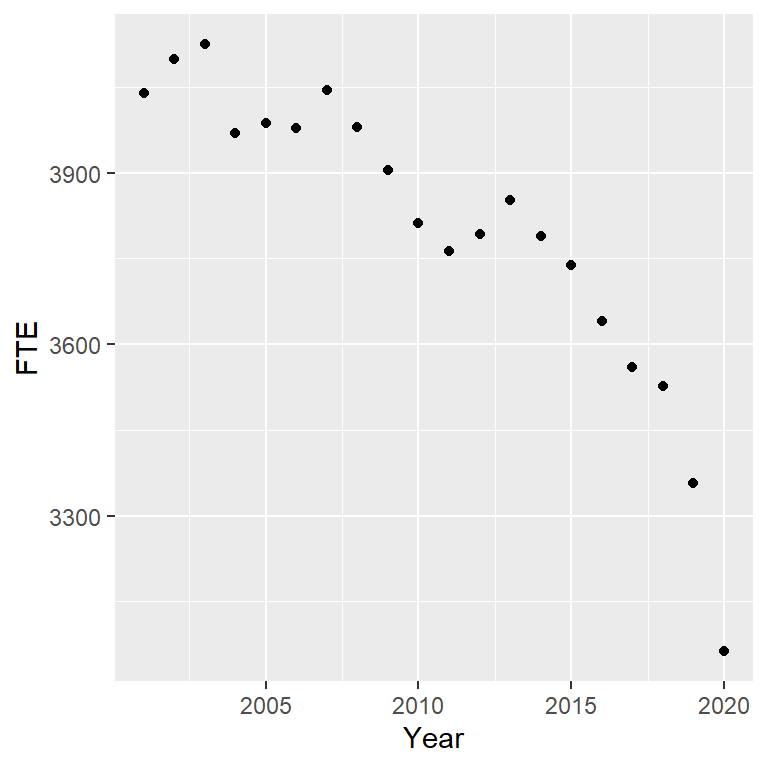
\includegraphics{Calvin-Mathematics_files/figure-latex/Last20-1} 

}

\caption{FTE Undergraduate Enrollment, 2000-2020}\label{fig:Last20}
\end{figure}

\hypertarget{statistics-for-a-new-century}{%
\section{Statistics For a New Century}\label{statistics-for-a-new-century}}

In some ways, statistics was to 2000 as computer science was to 1980 for the department. The department offered several statistics courses which were well-enrolled but had no PhD statisticians on the faculty and offered no major or minor in statistics.

The department offered four statistics courses in 2000. Mathematics 143 (now Stat 143), an introductory, algebra-based course, enrolled 348 students in 2000. This course was required in business and nursing programs and it also (since 1982) met the core requirement in mathematics. An introductory course such as this had been offered since 1936 and,from 1968 until 1990, a statistics course for business students that also included some finite mathematics was taught. Mathematics 243, introduced in 1983, enrolled 69 students in 2000. A calculus-based introduction to statistics, the course was a popular option for engineering students (as a mathematics elective) and mathematics majors. It was required of secondary education mathematics majors. Mathematics 343 and 344, a two-course sequence in mathematical statistics enrolled 16 and 5 students respectively in 2000. Math 343 was introduced by Sinke in 1960 and the second semester was added in 1979. Together, the department had three introductory courses taught at successively higher levels. All four of these courses are still being taught.

Discussions with the Engineering Department over the first few years of the century, centered on the Engineering Department's desire for their students to have a broader mathematics experience while at the same time not increasing the number of semester hours of course taking. In 2000, four courses (16 semester hours) in mathematics were required (three semesters of calculus and one of differential equations/linear algebra). The engineers wanted students to take some statistics and ABET accreditation standards expected that. Essentially, the engineers preferred a sophomore year of two courses (eight hours) that included vector calculus, differential equations, linear algebra, and statistics. This was informally dubbed the ``4 into 2'' problem. In 2003 the department introduced a course (Mathematics 232 - Engineering Mathematics) that attempted to address this need. The sophomore year for engineers then included the two courses Mathematics 231 and 232. Mathematics 232 contained about five weeks of statistics instruction.

\begin{figure}

{\centering 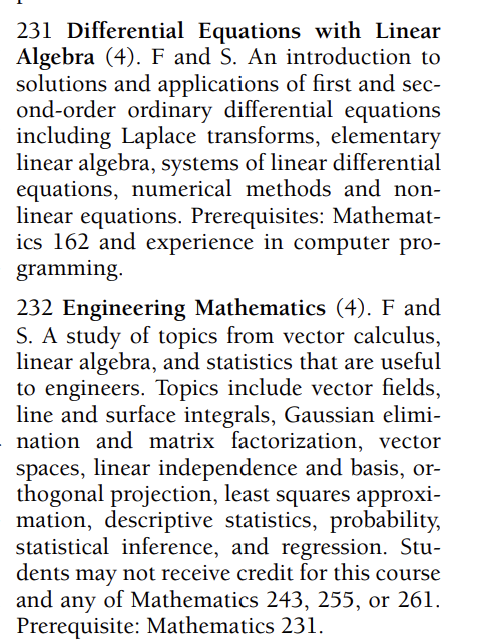
\includegraphics[width=6.67in]{images/M232} 

}

\caption{2003-2009 Second-year Courses for Engineers}\label{fig:M232}
\end{figure}

This sequence was offered from 2003-2009. The general consensus of both departments was that the sequence did not work well. This story is told more completely in a separate chapter. The resolution finally cam in 2010 when the departments agreed to split Mathematcs 232 into two courses: a more traditional vector calculus course (for 3 semester hours) and a new two-semester hour engineering statistics course. The mathematics cognate for engineers was thereby increased from 16 to 17 semester hours but the new courses (particularly vector calculus) were more focused and more successful.

To meet the needs of a different group, in 2009 the department introduced special sections of Mathematics 143 devoted to biostatistics. In that year, the Biology Department had begun requiring Mathematics 143 as a cognate to their major programs. (Eventually the special sections were offered under a new course number, Mathematics 145.)

Through 2014 it was still the case that students could take one of three different introductory courses in statistics (143, 243, 343) taught at progressively higher levels with progressively more demanding mathematical prerequisites. But a second course was only available to students taking Mathematics 343. In 2015, the department introduced a course, ``Applied Data Analysis'' (Statistics 245) that had a statistics prerequisite but not a calculus prerequisite giving many more students an opportunity to take a second course in statistics. (In 2015, the department also began designating statistics courses with the STAT rather than MATH designation although they were still housed in the mathematics department.) Finally, in 2016, the department began offering majors and minors in statistics having added two more courses at the 300-level -- a course in Bayesian Statistics (STAT 341) and a topics course in Statistics (STAT 385). At the same time, an interdisciplinary team launched a data science major and minors in data science and data analytics with three new courses taught under the DATA designation.

\hypertarget{faculty}{%
\section{Faculty}\label{faculty}}

There were 15 department members on tenure-track appointments in 2000. Two of these (Bradley and Fife) were on joint appointments with computer science. Of these 15, 9 would retire over the next 20 years and two would leave the college. So in 2020, just four of the faculty from 2000 remained (Ferdinands, Pruim, Scofield, and Turner). Due to the decrease in enrollment, there were just 10 faculty on tenure-track appointments in 2020, the four above joined by Bolt, Moseley, Kapitula, DeRuiter, Sunukjian, and Klanderman.

Just as it was difficult to hire computer scientists in the 1980s, it was, and remains, difficult to hire statisticians. Ph.D.~statisticians have many options, many of them more lucrative than college teaching. Additionally, academic statisticians often prefer to join a statistics department with an active community of statisticians. The problem of being the only or one of a few statisticians at an institution is known as the ``isolated statistician'' problem and there was even a listserve (ISOSTAT) for the community of such persons.

Just as mathematicians supervised and developed the computer science program in the 1980s, so did they supervise and develop the statistics program. The leader in these efforts was Randy Pruim. Trained as a logician, he shifted his efforts to statistics course and program development and even spent a sabbatical involved in a statistics research community at Michigan. His textbook for Mathematics 343 and 344 was ultimately published in a prestigious series of textbooks published by the American Mathematics Society. Several other department members taught statistics from time to time. The department was also fortunate in having Pam Plantinga and Barb Adams who faithfully taught Mathematics 143 on a parttime basis for many years. In fact, Plantinga taught at least four sections a year of that course for the entire period 2000-2020 we are describing here.

The department hired its first PhD statistician, Yousceek Jeong, in 1994. Unfortunately, Jeong stayed just two years. Kathyrn Jacobsen, an epidemiologist, was hired by the Biology Department in 2005 with the expectation that she would also teach statistics but she stayed only two years. Laura Kapitula was hired in 2009 but she also stayed just three years. Stacy DeRuiter, whose PhD program in Biological Oceanography at MIT contained a lot of statistics, joined the department in 2013 and still serves as the only real statistician in the department.

The retirements of Koop and Talsma in 2018 also made hiring for mathematics education a priority. Dave Klanderman joined the department in 2019 from Trinity Christian College where he had spent many years. With just one person in mathematics education, the department was fortunate that Talsma and Koop stayed on to teach parttime on occasion.

\hypertarget{the-rinck-prize}{%
\chapter{The Rinck Prize}\label{the-rinck-prize}}

The Rinck Prize, named after the first mathematics professor, William Rinck, is the oldest prize in the college. Professor Rinck was 43 years old when he died in an automobile accident along with his young son. Professor Rinck was well-like by his students and his colleagues and over the next few years they contributed \$500 that was used to set up a fund to award a prize to an outstanding mathematics student. The fund has grown over the years so that the award is substantial and, aided by an additional substantial donation from Professor Rinck's daughter, the fund fund now also supports a scholarship.

The first award was given in the spring of 1928. It was awarded to John A. Bolt, a junior student from Raymond, MN. Bolt went on to a career as a chemist in the Chicago area. The catalog description of the prize doesn't suggest any particular criteria.

\begin{figure}

{\centering \includegraphics[width=0.7\linewidth]{images/Rinck1927} 

}

\caption{1927 catalog description of Rinck Prize}\label{fig:Rinck}
\end{figure}

By 1930, the catalog describes the criteria in terms of performance in five courses: college algebra, two semesters of analytic geometry, and two semesters of calculus.

\begin{figure}

{\centering \includegraphics[width=0.7\linewidth]{images/Rinck1930} 

}

\caption{1930 catalog description of Rinck Prize}\label{fig:Rinck30}
\end{figure}

The criteria remained the same until 1961 when the department revised the curriculum so that well-prepared students started in calculus. Analytic geometry was no longer required (or offered). The criteria changed to the current statement.

\begin{figure}

{\centering 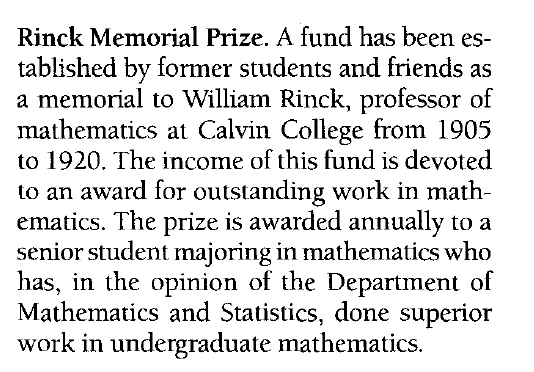
\includegraphics[width=0.6\linewidth]{images/Rinck2000} 

}

\caption{Current catalog description of Rinck Prize}\label{fig:Rinck00}
\end{figure}

The criteria are, of course, quite open-ended and the faculty often have spirited discussions in trying to determine the winner each year. In the early years, with fewer faculty, all faculty knew all students well and the criteria emphasized performance in five specified courses. As the faculty and number of courses offered grew, it became more difficult to compare the performance of individual students. The department also began to consider performance of students outside the classroom such as in independent research and participation in the colloquium.

One of the consequences of offering a rich set of mathematical electives is that some students take more courses than others. For example, the secondary education mathematics students take a minimal major due to the number of other professional courses that they must take to complete the program (including a whole semester of directed teaching). Also, double majors usually take fewer mathematics courses. The introduction of the Paul Boonstra Memorial Award given to a graduate senior specializing in mathematics education allowed the department to address this first group of students. Paul Boonstra was the first faculty member speicializing in mathematics education.

\begin{figure}

{\centering 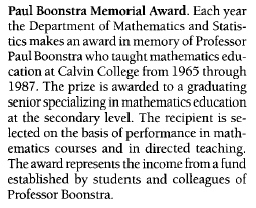
\includegraphics[width=0.6\linewidth]{images/Boonstra} 

}

\caption{Current catalog description of Paul Boonstra Memorial Award}\label{fig:Boonstra}
\end{figure}

The list of winners over time gives some insight into the role of mathematics at Calvin over the years. Many of the early winners of the award were not considered mathematics majors. And, since the award was based on coursework through calculus, many non-majors won the prize. Engineering students were prime candidates. Gordon Van Wylen (1940), who would later go on to become the President of Hope College, was an engineering student who completed his engineering degree at Michigan. In the late 1930s and throughout the 1940s, the award usually wnet to a chemistry major. Enno Wolthuis (1931) Ted Dirkse (1935) were first award winners to come back to Calvin as faculty members. They served the department of chemistry until their retirements. The appeal of chemistry in the 1940s was in large part due to the presence of John (``Doc'') DeVries who had a PhD and a research program. DeVries Hall is named after ``Doc'' DeVries in honor of his outsized influence on Calvin. Rinck winners of the 1940s inlcuded Charles Dekker (1941) who would have a career as a UC Berkeley chemistry faculty member, John Huizinga (1943) who became an Argonne National Laborator chemist and later received the Calvin College distinguished alumni award, and Calvin professor Herman Broene (1942). Other chemistry professors from this era who won the award include Russel Maatman (1946), Anne DeBoer Deckard (1945), and Harold Van Kley (1953).

The addition of the requirement in 1961 that the prize winner be a mathematics major changed this pattern of chemists winning the award. However, often the winner was a double major. In the early 1970s winners included Steve Haan (1973) who would have a career as a physicist at Lawrence Livermore Lab, and David Cok (1975) who, after receiving a Harvard PhD in Physics, would have a career at Kodak. Chemistry students continued to win the award at a regular clip. Recent award winners who have gone on to pursue chemistry PhDs include Andrea Bootsma (2015) and Grace Johnecheck (2019). Philosophy double major Eddy Chen (2013) is currently a philosophy professor. After the introduction of the computer science major in 1980, several winners were computer scientists including Jack Snoeyink (1985) who received a Stanford PhD in Computer Science and teaches at North Carolina nad Ethan Van Andel (2011) who received a Berkeley PhD and is a software engineer.

Of course a typical career path for a Rinck Prize winner is to earn a PhD in mathematics and to have a career as a mathematics professor. Besides Zwier, Tom Jager (1966), Mike Stob (1974), Wayne Dyksen (1977), Randy Pruim (1988), and Mike Bolt (1994) returned to teach at Calvin. Curiously, three of these (Jager, Stob, and Bolt) received their PhD from Chicago. Dyksen taught at Calvin for three years before moving on to Purdue and, eventually MSU as a computer science professor. Other mathematics PhDs include Ward Bouwsma (1956) who would eventually become an editor of Mathematical reviews, Bob Daverman (19) who served as Associate Secretary of the AMS for many years and won the Calvin distiguished alumni award, and several winners who are still active mathematics professors. PhD statisticians who have won the award include Sharon Lohr (1982), a Fellow of the American Statistical Association, and Paul Vos (1983).

Perhaps mathematics runs in families. Randy Pruim (1988) and his son Jason (2021) are winners. So are Jack Snoeyink (1985) and his daughter Sarah Snoeyink Van Fossen (2010). Tom Jager (1966) along with all three of his daughters Rebekah Jager Arana (1995), Abby Jager (1998), and Leah Jager (2001) were Rinck Prize winners. All three Jager women received PhDs, Rebekah in mathematics from Notre Dame and Abby and Leah in statistics. Evelyn Van Appledorn Oostendorp (1934) was the grandmother of William Oostendorp (1987)!

\hypertarget{research-in-the-mathematics-department}{%
\chapter{Research in the Mathematics Department}\label{research-in-the-mathematics-department}}

\hypertarget{faculty-research}{%
\section{Faculty Research}\label{faculty-research}}

In the 1980s, the department and the college began to place increased emphasis on faculty research both in hiring and in decisions on reappointment and tenure. While there were several faculty members engaged in scholarship as early as the 1940s (John DeVries in Chemistry, for example), it is fair to say that having an active research program was not a requirement for tenure and not necessarily an important criteria in hiring. This varied quite a bit by department.

The mathematics department began hiring PhDs in 1960 and every tenure-track hire after that (except for Jack Kuipers) had a PhD. But it is fair to say that the department made a push to hire faculty with active research programs only beginning with the hires of Venema (1979) and Stob (1981). Venema and Stob each came to the college from postdoctoral research positions and with NSF grants in hand.

While individual departments varied in their emphasis on faculty research, the college began in the early 1980s to institute programs to support and encourage faculty research. The most important and effective of these was the Calvin Research Fellowship (CRF) program. A CRF was a reduction in teaching load to provide time for a faculty member to pursue a scholarly project. The program started modestly in 1982 with just five course reductions college-wide. Stob and Venema were each awarded one. The program quickly grew and over the years many department members have had multiple ``units'' of CRFs.\\
Also, in the 1980s, the college placed more emphasis on the notion that a sabbatical was for support of a scholarly project and not just for a semester of relief. In turn, the college tried to fund the sabbatical program at a high level so that all worthy sabbatical projects would be funded. These two programs - the CRF program and a robust sabbatical program - remain important and effective tools for supporting faculty research.

Besides the internal suppport for research, the college gradually devoted more support and encouragement for faculty to pursue external funding. It is fair to say that in the 1980s, the college still did not support faculty with grants well. Faculty were expected to do their own grant accounting and to find their own sources of funding. By the late 1990s however, the college provided considerable more support for faculty to apply for grants including the creation of a Dean for Research position and an office of Grants and External Programs with personnel to help navigate funding agency requirements. Several mathematics faculty over the years have had substantial external support from agencies such as NSF, the Michigan Department of Education, and the John Templeton Foundation.

\hypertarget{departmental-statement-on-research}{%
\section{Departmental Statement on Research}\label{departmental-statement-on-research}}

In 1991, the \{\em ad hoc\} Committee on Faculty Research sent to the Professional Status Committee entitled \{\em Research and Scholarship: the Responsibilities of the Faculty.\} That committee was appointed as a result of the 1987 college strategic plan that called for investment in faculty research. The \{\em ad hoc\} committee determined the need to define more carefully what was to be expected of faculty in the area of research and scholarship. The Professional Status Committee, upon the recommendation of the \{\em ad hoc\} committee, noted that the nature of and expectations for research did and probably should vary by department and mandated that departments create statements on research that addressed four questions:

\begin{enumerate}
\def\labelenumi{\arabic{enumi}.}
\tightlist
\item
  What do research and scholarship mean in that department?
\item
  How do research and scholarship contribute to the mission of
  the college?
\item
  What methods should be used to evaluate research
  and scholarship of members of the department? and
\item
  What means will the department use to promote research and scholarship?
\end{enumerate}

Under the leadership of Gerard Venema, the college created a statement that, with some light revision, still serves the department well today. The two major features of that statement are its responses to question 1 and 3.

The department chose to use a broad definition of research and scholarship. So, while traditional research such as that supported by the NSF was included, so were research programs that concerned pedagogy or Christian perspectives on mathematics. The statement however emphasized that ideally any such program should result in publication, broadly conceived, to an external audience.

The department also established a method of evaluating research. At each reappointment occasion, the department appoints a two person committee to evaluate (and give feedback on) the research program of the faculty member. At the same time, the department also established a similar process of a two-person committee evaluating teaching. These committees, when they work worked well helped the candidate understand better the expectations of the department.

\hypertarget{student-research}{%
\section{Student Research}\label{student-research}}

By the 1980s, it was not uncommon for there to be students engaged in research projects in the summer, especially in the chemistry and physics department. These projects were normally funded by external grants. In the late 1980s, the science division began to provide funds to support such students and this has grown into a large program of student summer research. Funds come from several endowments and occasionally some division-wide external grants.

The department's first foray into summer student research was through a Research Experience for Undergraduates (REU) grant from the NSF. This grant was joint with Hope College and it allowed Stob and Venema to support students during the summer of 1992. Students were selected to participate in the Hope-Calvin program from external applicants and from Calvin and Hope students. Half the students had to be from outside the two institutions. The summer program had a component of instruction (with some external speakers), social activities, and research. Stob and Venema each had a non-Calvin student as well as one or two Calvin students. Stob's student Tom Nevins, a Notre Dame undergraduate, had particular success. His summer project resulted in a publication in a peer-reviewed journal. Nevins would go on to graduate school at Chicago and a career at Illinois. Nevins in fact proved the opposite of what Stob expected would be the result of the project. While Hope continued the REU, Stob and Venema only participated that first year.

As science division funds increased and faculty members received external grants that funded student research, several faculty routinely supervised Calvin students in summer research projects. Several of these student projects resulted in publications and some students presented at meetings such as MathFest or the Michigan Section of the MAA.The department also encourages students to apply for off-campus research positions in the summer. The availability of such positions greatly increased over the past 20 years due to the significant expansion of the REU program. The culmination of a summer research position is a poster presentation at the annual science division poster session in the fall. Students from across the division prepare a poster that is displayed in the lobby of DeVries Hall. Students are available to answer questions about their posters.

\hypertarget{mathematics-and-engineering}{%
\chapter{Mathematics and Engineering}\label{mathematics-and-engineering}}

Calvin has always had an engineering program. In 1920, students studied two years at Calvin before finishing their degree at an engineering school, usually the University of Michigan. By the 1940s, the program had become what is commonly called a 3+2 program -- three years at Calvin and two at an engineering school. Calvin even gave an undergraduate degree to students who completed such a 3+2 progam. In 1985, Calvin offered a four-year engineering program for the first time that resulted in a BSE degree. In most years of Calvin's existence (all except perhaps some years during the 1970s) there were actually more engineering students in each class than mathematics majors. By the laste 1990s, over 100 first-year students would start the engineering program each year although not nearly so many would complete it.

Since engineering students always took at least four courses in the department, the department always needed to negotiate the content and scheduling of those courses with the engineering department. While in general these negotiations were collegial, at times they caused the department to make compromises that were uncomfortable. One challenge is that most courses that engineering students take serve other students as well, including mathematics majors, and their needs cannot be ignored. This challenge became greater as the number of engineering students greatly increased in the 1980s and as the engineering department felt more pressure from its accreditation agency, ABET, to include certain topics in the curriculum.
Besides the challenge of providing mathematics courses that fit the engineering program, another challenge has always been the wide range of preparation of engineering students in mathematics.

\hypertarget{the-mathematics-curriculum-for-engineering-students}{%
\section{The Mathematics Curriculum for Engineering Students}\label{the-mathematics-curriculum-for-engineering-students}}

From 1920, when the college offered a four-year program, until 1985 when the engineering program first offered a four year degree, pre-engineering students and mathematics majors took the same four-course introductory sequence in mathematics. Before 1961, that included two semesters of analytic geometry and two semesters of calculus. By the late 1950s, the engineering program would also require a differential equations courses resulting in a five-course mathematics cognate. After 1961, three semesters of calculus and one semester of differential equations would be the standard first- and second-year sequence. A technical elective provided a possible fifth mathematics course.

The BSE degree, introduced in 1985, continued to require the four-course package of calculus and differential equations and also required students to take an ``advanced mathematics elective''. That elective was usually chosen from among statistics, partial differential equations, and complext variables but engineers sometimes chose other courses for this elective (such as abstract algebra) particularly if they wanted to minor in mathematics (by taking a sixth course). Since by 1985, the third course in calculus and the differential equations course were not required of mathematics majors, engineering students formed the majority in these courses.

By the early 2000s, the engineering department was addressing a perceived pressure to include more engineering courses in its program as well as to include more topics in its mathematics cognate. Specifically, the engineering department asked the mathematics department to offer a four-course sequence that addressed all the topics of the three semester calculus sequence, differential equations, linear algebra, and statistics. After a long negotiation, a four-course sequence acceptable to the enginnering department was implemented in 2003. This sequence included the standard calculus I course, a calculus II course that included some topics previously included in calculus III, a sophomore ``engineering mathematics'' course that was approximately 8 weeks of multivariable caclulus and five weeks of statistics, and a differential equations/linear course.

The department offered this four course sequence for six years. However, it became clear from the very beginning that there were some serious difficulties with this sequence. One problem was that the new calculus II was now ``nonstandard.'' Not only did this make the course more difficult for students but it also presented problems for advanced placement students. Students who completed the BC syllabus and normally would be placed in calculus III were now missing some topics and had a more difficult time starting in that course. A more serious problem was that the statistics/multivariable calculus course proved to be quite difficult to teach. It was difficult to construct a syllabus for (or find a textbook for) the statistics portion and it was difficult to do enough multivariable calculus to prepare the engineering students for the physics cognate.

In 2010, the two departments agreed on revisions to the sequence. The Calclus II course reverted to a more standard course. A standalone statistics course was created for engineers. While this course was only a two-semester hour course, it still had a substantially greater coverage of statistics than was possible in the engineering mathematics course and, since it was a standaloIt also provided the opportunity for engineers to take a four hour statistics course to meet the statistics cognate if they had room in their program (for example, if they had AP calculus credit). The multivariable calculus course was reinstated but a three-semester hour version was introduced. This was done by teaching the standard multivariable calculus course (which was four hours) but arranging topics so that engineering students could leave the course after 10 weeks with the what was necessary to proceed in the program. Effectively, this changed the cognate requirement from 16 semester hours to 17 semester hours.

\hypertarget{the-mathematical-preparation-of-engineering-students}{%
\section{The Mathematical Preparation of Engineering Students}\label{the-mathematical-preparation-of-engineering-students}}

Since 1961, the mathematics cognate for the Engineering program has included three semesters of Calculus. By 1966, the engineering program was constructed assuming that students took Calc I in the first semester of the first year. But not all engineering students are equally ready for Calc I. Of course, this is not particularly an engineering student problem but it is particularly consequential for engineering students due to the prerequisite structure of the program. Students who don't start Calc I in the first semester of their first year usually need a full extra year to complete the program (either the 3+2 program of 1961-1985 or the four-year degree program started in 1985). The mathematics department has used various strategies over the year to place students in an appropriate mathematics course and to construct pathways that might allow students to ``catch-up'' to their classmates who started in Calc I.

From 1961 until 1991, the prerequisite for Calc I was expressed in various ways but was essentially two years of high school algebra and at least a semester of high school trigonometry. Along with the expected course in geometry, this resulted in an expectation of 3.5 years of high school mathematics. Many students, especially in the early years of this period, came from high schools that did not offer a fourth year of high school mathematics. Many others elected not to take that fourth year of mathematics in lieu of other electives at the high school. It was not necessarily the case that high school students expecting to study engineering realized the amount of mathematics that they would need to take. Throughout this period, the department offered courses in algebra and trigonometry (sometimes in two separate courses and sometimes in one combined course) so that students could start calculus in the spring of their first year or the fall of their second year. By 1979 this course was called Precalculus Mathematics (110) and was listed as an alternative prerequisite to Calc I. Again, students taking this path were effectively a year behind in the three year program

In 1982, the department began offering Calc I (Mathematics 161 at the time) during the interim term. This gave engineering students the possibility of ``catching up'' to their cohort by taking Mathematics 110 in the fall and calculus during the interim. Calculus in 15 days was challenging. The course met 8:30-5 and included both lecture sessions and supervised homework sessions. Usually two instructors were assigned to teach it. The success rate of students in this track was not great.

By 1992, more students were coming to Calvin with four years of high school mathematics and the department realized that students with four years of mathematics in high school were in general more successful in the course. The department formally set the the prerequisite for calculus to be four years of high school mathematics and the prerequisite for pre-calculus to be three years of high school mathematics. Realizing that not all high schools are equal, the department also instituted a placement test that students with four years of high school mathematics took during the orientation period before classes began. The department created a version of Calculus that was one and one-quarter course units for students deemed by the placement test to be not quite ready for calculus. Thus there were two pathways for those not prepared for the standard Calc I course (161). Students could either take 110 in the fall and then 161 during the interim or take 160 in the fall.

In 1998, the department determined that Mathematics 160 was not sufficient to make students ready for Mathematics 162 (Calc II). Therefore the department created a two-course sequence, 159 and 160 to be taken during the fall and interim terms to be a pre-calculus/calculus I sequence for those students who had four years of high school mathematics but were deemed by the placement test not to be ready for 161. The department also stopped teaching 161 in the interim thereby determining that there was no path for students to catchup who started in pre-calculus. These changed were made after examining the performance of students who started in 110 - essentially none of these students were successful in catching up and completeing the four-year engineering program on time. The department stopped offering 110 in 2015.

The department stopped offering the fall-interim sequence of pre-calculus in 2020. Instead, students with four years of high school mathematics entered Calc I. However, a new one-hour course called Calculus I supplemental instruction was offered to be taken alongside Calc I. Just 12 students enrolled that first year. In 2021, the college eliminated the interim term so the strategy of using interim to catch up is not available anyway.

It is fair to say that the above story has two themes that are constantly in tension. The first is the increasing acknowledgement that success in calculus demands a solid four-year high school preparation (or its equivalent). The second is that starting in anything other than Calculus I is deemed very undesirable for engineering students. The departments attempts to enforce the former while acknowledging the latter led to a variety of strategies for placement and curriculum.

\hypertarget{the-mathematics-major-1}{%
\chapter{The Mathematics Major}\label{the-mathematics-major-1}}

This section is an attempt to document all the changes in the requirements for a mathematics major over the first 100 years of the department. The department has had a major since 1920 and a major for secondary education students since 1967. Here we describe all the changes in each of these two. Additionally, the department has had a major for elementary education students, a statistics major, an actuarial science major, and, with computer science, a data science major.

\hypertarget{the-1920-1926-major}{%
\section{The 1920-1926 Major}\label{the-1920-1926-major}}

In 1920, students really didn't major in mathematics but rather completed a group major in the so-called Group II: Mathematics, Physics, Chemistry, Zoology, Botany, Psychology, and Logic. Within this group students needed to take four semester courses of three hours each in two departments. So a mathematics major would be considered 12 hours in at least four courses. Two courses in analytic geometry and two in calculus would be the normal way to complete this requirement (although it would comprise 16 hours).

\hypertarget{the-1927-1948-major}{%
\section{The 1927-1948 Major}\label{the-1927-1948-major}}

In 1927, the major requirements were revised but still used the group framework. Logic was removed from the group. Students were required to take 36 hours in their major group with at least 21 hours in one of the departments of that group (and 12 in another). The two departments were called the major and minor departments of the major group. So a mathematics major would consist of 21 hours of courses. The analytic geometry and calculus courses comprised 16 of these hours. Additional electives included differential equations, theory of equations, and solid analytic geometry.

\hypertarget{the-1949-1966-major}{%
\section{The 1949-1966 Major}\label{the-1949-1966-major}}

In 1949, using the same framework, the requirement remained at 36 hours total for the major group but the student was required to take 24 hours (instead of 21) in one of the departments.

\hypertarget{the-1967-major}{%
\section{The 1967 Major}\label{the-1967-major}}

With the change to the 4-1-4 curriculum, 1967 was the first year that departments specified the requirements for their own programs of concentration (which was what majors were called).

The mathematics major was eight courses: three semesters of calculus, differential equations, abstract algebra, and three 300-level electives. The department also specified the secondary education mathematics major to include geometry, statistics, and topology (!) as the three 300-level electives, and also to include an interim course in mathematics. Perhaps topology was a typo. In any event, that particular requirement was changed the very next year.

\hypertarget{the-1968-1981-major}{%
\section{The 1968-1981 Major}\label{the-1968-1981-major}}

In 1968, the department made two changes. An interim course was added to the requirements for the general major (making the major nine courses). The topology requirement was changed to a history of mathematics requirement in the secondary education major. The history of mathematics course was new that year and certainly a better option than topology.

\hypertarget{the-1982-1990-major}{%
\section{The 1982-1990 Major}\label{the-1982-1990-major}}

The 1982 revision to the major opened up the sophomore year and also provided some structure to the choice of 300-level electives. The major included two semesters of calculus, two 200-level mathematics courses, two semesters of the non-credit colloquium, a interim course, and four 300-level courses. The 300-level courses were required to include: a course in algebra, a course in analysis, a course emphasizing applications, and a course emphasizing formal proof. A computer science cognate was also added. (At that time it was a course in Pascal programming.)

The requirements for secondary education students were considerably revised. They simply included two semesters of calculus and seven 200- and 300-level courses chosen with the approval of the advisor. The catalog was eventually edited to indicate that an upper-level mathematics interim course could be included among those seven. Education 356 substituted for the colloquium requirement of the general major.

\hypertarget{the-1991-2003-major}{%
\section{The 1991-2003 Major}\label{the-1991-2003-major}}

The rather complicated description of the requirements of the general major of the previous nine years caused the department to simplify the statement of the major in 1991. The mathematics major was still eight courses, an approved interim, two semesters of the colloquim, and a computer science cognate. But the eight courses were: two semesters of calculus, two 200-level courses, real analysis, abstract algebra, and two additional 300 level courses.

The secondary education sequence was completely specified. It followed the same form as the general major but the two 200-level courses were specified as statistics (MATH 243) and applied linear algebra (MATH 255). The four 300-level courses were abstract algebra, analysis, history of mathematics, and geometry.

\hypertarget{the-2004-2019-major}{%
\section{The 2004-2019 Major}\label{the-2004-2019-major}}

With the change from the course unit system to the semester hour system in 1997, the department had been introducing some 3-hour courses while most courses were 4-hours. In 2004, the department changed both the general and secondary education sequence in a way that hours mattered.

In the general major, the department specified that one of the 200-level courses be MATH 256 which was a discrete mathematics/linear algebra combination designed partly with the needs of computer science majors in mind. (In 2017, the requirement would be replaced by MATH 255, an applied linear algebra course) The other 200-level course was chosen from a third semester of calculus, differential equations, or statistics (MATH 243). Four courses were still required at the 300-level including real analysis, abstract or linear algebra, and two courses of at least 7 hours from other 300-level electives.

The secondary education major was changed by substituting MATH 256 for linear algebra, adding MATH 329 (a two-hour course called introduction to teaching secondary school mathematics) and by changing the history requirement to the new perspectives in modern mathematics course (which ahd a strong historical component).
MATH 329 would be replaced by MATH 327, essentially the same course but focusing on middle school, in 2018.

\hypertarget{courses}{%
\chapter{Courses}\label{courses}}

The following table lists the department's courses as of Fall, 2020. The table includes the first year that the course was offered, its orginal number, and its original title. Courses evolve over time and so the original version of a course might not bear much resemblance to its current version. Furthermore, there are a few instances where the current course might not bear any relation to its ``predecessor.'' For example, MATH 333 (PDEs) has no content in common with MATH 311 (introduced in 1961) though it definitely came from MATH 311 via incremental year-over-year changes. Omitted are the computer science courses, many of which orginated in the department.

\begin{table}

\caption{\label{tab:willem}2020 Courses and their Origins}
\centering
\begin{tabular}[t]{llrll}
\toprule
Number & Title & Orginal Year & Original Number & Orginial Title\\
\midrule
MATH 071 & Calculus I Supplemental Instruction & 2020 & MATH 071 & Calculus I Supplemental Instruction\\
MATH 072 & Calculus II Supplemental Instruction & 2020 & MATH 072 & Calculus II Supplemental Instruction\\
MATH 100 & Mathematics in the Contemporary World & 1962 & MATH 109 & Elements of Modern Mathematics\\
MATH 132 & Calculus for Management & 1948 & MATH 205 & Business Mathematics\\
MATH 171 & Calculus I & 1920 & MATH 7 & Differential and Integral Calculus\\
\addlinespace
MATH 172 & Calculus II & 1920 & MATH 8 & Continuation of Course 7\\
MATH 190 & First Year Seminar in Mathematics & 1998 & MATH 190 & First-Year Seminar in Mathematics\\
MATH 221 & The Real Number System and Methods for Elementary School Teachers & 1979 & MATH 107 & Fundamental Concepts in Mathematics: the real number system\\
MATH 222 & Geometry, Probability, Statistics, and Methods for Elementary School Teachers & 1979 & MATH 209 & Fundamental Concepts in Mathematics: Geometry\\
MATH 231 & Differential Equations with Linear Algebra & 1923 & MATH 9 & Differential Equations\\
\addlinespace
MATH 251 & Discrete Mathematics & 1979 & MATH 251 & Discrete Structures\\
MATH 252 & Discrete Mathematics for Computer Science & 1998 & MATH 156 & Discrete Mathematics for Computer Science\\
MATH 255 & Introductory Linear Algebra & 1982 & MATH 255 & Applied Linear Algebra\\
MATH 270 & An Introduction to Multivariable Calculus & 2010 & MATH 270 & An Introduction to Multivariable Calculus\\
MATH 271 & Multivariable Calculus & 1961 & MATH 211 & Calculus and Analytic Geometry\\
\addlinespace
MATH 301 & Foundations of Geometry & 1962 & MATH 320 & Foundations of Geometry\\
MATH 305 & The Geometry and Topology of Manifolds & 1966 & MATH 361 & General Topology\\
MATH 312 & Logic, Computability, and Complexity & 1978 & MATH 381 & Advanced Logic\\
MATH 323 & Teaching Mathematics in the Elementary and Middle School & 2010 & MATH 323 & Teaching Mathematics in the Elementary and Middle School\\
MATH 327 & Mathematics Content and Teaching Methods for Middle Grades & 2019 & MATH 327 & Mathematics Content and Teaching Methods for Middle Grades\\
\addlinespace
MATH 331 & Nonlinear Dynamics and Chaos & 2011 & MATH 331 & Nonlinear Dynamics and Chaos\\
MATH 333 & Partial Differential Equations & 1961 & MATH 311 & Advanced Analysis\\
MATH 335 & Numerical Analysis & 1967 & MATH 335 & Numerical Mathematics\\
MATH 351 & Abstract Algebra & 1960 & MATH 309 & Introduction to Modern Algebra\\
MATH 355 & Advanced Linear Algebra & 1967 & MATH 352 & Abstract Algebra\\
\addlinespace
MATH 359 & Seminar in Secondary Teaching of Mathematics & 1969 & EDUC 356 & Seminar in Secondary Teaching Methods\\
MATH 361 & Real Analysis I & 1968 & MATH 362 & Real Analysis\\
MATH 362 & Real Analysis II & 1982 & MATH 362 & Real Analysis II\\
MATH 365 & Complex Variables & 1962 & MATH 312 & Advanced Analysis\\
MATH 380 & Perspectives on Modern Mathematics & 2004 & MATH 380 & Perspectives on Modern Mathematics\\
\addlinespace
MATH 383 & External Practicum & 2020 & MATH 383 & External Practicum\\
MATH 390 & Independent Study & 1967 & MATH 400 & Readings in Mathematics\\
MATH 391 & Colloquium & 1982 & MATH 391 & Colloquium\\
MATH 395 & Senior Thesis in Mathematics & 1974 & MATH 395 & Senior Thesis in Matheamtics\\
STAT 143 & Introduction to Probability and Statistics & 1979 & MATH 241 & Elementary Statistics\\
\addlinespace
STAT 145 & Biostatistics & 2012 & MATH 145 & Biostatistics\\
STAT 241 & Engineering Statistics & 2010 & MATH 241 & Engineering Statistics\\
STAT 243 & Statistics & 1982 & MATH 243 & Statistics\\
STAT 245 & Applied Data Analysis & 2015 & STAT 245 & Applied Data Analysis\\
STAT 341 & Computational Bayesian Statistics & 2016 & STAT 341 & Computational Bayesian Statistics\\
\addlinespace
STAT 343 & Probability and Statistics & 1960 & MATH 308 & Mathematical Statistics\\
STAT 344 & Mathematical Statistics & 1979 & MATH 344 & Mathematical Statistics\\
STAT 383 & External Practicum & 2020 & STAT 383 & External Practicum\\
STAT 390 & Independent Study & 1967 & MATH 400 & Readings in Mathematics\\
\bottomrule
\end{tabular}
\end{table}

\hypertarget{department-faculty}{%
\chapter{Department Faculty}\label{department-faculty}}

There have been 41 tenured or tenure-track faculty in the department. (Here we include the first four faculty members who were appointed before tenure was a thing at Calvin.)

\begin{table}

\caption{\label{tab:faculty}Tenured and Tenure-Track Department Faculty}
\centering
\begin{tabular}[t]{lllllrrll}
\toprule
Last & First & Calvin Grad & Degree & Institution & Year & Started & Ended & Status at end\\
\midrule
Rinck & William &  & MA &  &  & 1920 & 1920 & died\\
Nieuwdorp & James &  & BS &  &  & 1920 & 1944 & retired\\
Muyskens & Albert & Yes & MA &  &  & 1941 & 1961 & retired\\
Tuls & John & Yes & MA & Michigan & 1944 & 1946 & 1972 & retired\\
Sinke & Carl & Yes & PhD & Purdue & 1954 & 1956 & 1991 & retired\\
\addlinespace
Zwier & Paul & Yes & PhD & Purdue & 1960 & 1960 & 1996 & retired\\
Nyhoff & Larry & Yes & PhD & Michigan State & 1969 & 1964 & 2002 & to CS\\
Boonstra & Paul & Yes & PhD & Michigan State & 1970 & 1965 & 1987 & died\\
Kuipers & Jack & Yes & MSE & Michigan State & 1966 & 1967 & 1986 & retired\\
Van Zwalenberg & George & Yes & PhD & California Berkeley & 1968 & 1968 & 1999 & retired\\
\addlinespace
Leestma & Sanford & Yes & PhD & New Mexico St & 1969 & 1968 & 2003 & retired\\
Jager & Thomas & Yes & PhD & Chicago & 1971 & 1974 & 2011 & retired\\
Brink & Daryl & Yes & PhD & Michigan State & 1973 & 1976 & 2007 & retired\\
Venema & Gerard & Yes & PhD & Utah & 1975 & 1979 & 2016 & retired\\
Stob & Michael & Yes & PhD & Chicago & 1979 & 1981 & 2018 & retired\\
\addlinespace
Dyksen & Wayne & Yes & PhD & Purdue & 1982 & 1982 & 1985 & left\\
Klaasen & Gene &  & PhD & Nebraska & 1968 & 1984 & 1992 & left\\
Laverell & W David &  & PhD & Lehigh & 1969 & 1984 & 2001 & retired\\
Talsma & Gary & Yes & PhD & Purdue & 1986 & 1984 & 2018 & retired\\
Bradley & James &  & PhD & Rochester & 1974 & 1986 & 2007 & retired\\
\addlinespace
Ye & Xiang Dong &  & PhD & Iowa & 1987 & 1987 & 1998 & left\\
Fife & Earl &  & PhD & Wesleyan & 1977 & 1988 & 2014 & retired\\
Ferdinands & R John &  & PhD & Purdue & 1988 & 1988 & current & current\\
Koop & Janice & Yes & PhD & Colorado & 1978 & 1989 & 2018 & retired\\
Adams & Joel &  & PhD & Pittsburgh & 1988 & 1989 & 2022 & to CS\\
\addlinespace
Vander Linden & Keith &  & PhD & Colorado & 1993 & 1990 & current & to CS\\
Jeong & Yousceek &  & PhD & Michigan & 1993 & 1994 & 1997 & left\\
Pruim & Randall & Yes & PhD & Wisconsin & 1995 & 1997 & current & current\\
Scofield & Thomas &  & PhD & Michigan State & 1998 & 1998 & current & current\\
Wagstrom & Rikki &  & PhD & Nebraska & 1999 & 1999 & 2005 & left\\
\addlinespace
Turner & James &  & PhD & MIT & 1994 & 1999 & current & current\\
Hanisch & Mark &  & PhD & Cornell & 1991 & 1999 & 2006 & left\\
Bolt & Michael & Yes & PhD & Chicago & 2001 & 2004 & current & current\\
Moseley & Christopher &  & PhD & North Carolina & 2001 & 2006 & current & current\\
Myers & Marilyn &  & PhD & Queens & 2007 & 2007 & 2014 & left\\
\addlinespace
Kapitula & Todd &  & PhD & Maryland & 1991 & 2007 & current & current\\
Kapitula & Laura &  & PhD & New Mexico & 2002 & 2009 & 2012 & left\\
DeRuiter & Stacy &  & PhD & MIT & 2008 & 2013 & current & current\\
Jung & Hyunyi &  & PhD & Indiana & 2011 & 2015 & 2017 & left\\
Sunukjian & Nathan &  & PhD & Michigan State & 2010 & 2016 & current & current\\
\addlinespace
Klanderman & David & Yes & PhD & Northern Illinois & 1996 & 2020 & current & current\\
\bottomrule
\end{tabular}
\end{table}

  \bibliography{book.bib,packages.bib}

\end{document}
